%%%%%%%%%%%%%%%%%%%%%%%%%%%%%%%%%%%%%%%%%%%%%%%%%%%%%%%%%%%%%%%%%%%%%%%%%%%%%%%%%%%%%%%%%%%%%
%% Poster A0 portrait template University of Tübingen
%
% created by Ekaterina Kohler (ekaterina.kohler@googlemail.com)
% 2022/03/07: completely revised by Chris Nill (chris.nill@student.uni-tuebingen.de)
%
%%%%%%%%%%%%%%%%%%%%%%%%%%%%%%%%%%%%%%%%%%%%%%%%%%%%%%%%%%%%%%%%%%%%%%%%%%%%%%%%%%%%%%%%%%%%%

\documentclass[a0,plainsections]{sciposter}
\usepackage{posterA0} % is located in the same folder as this file and contains all packages and settings

%% your personal packages
%%%%%%%%%%%%%%%%%%%%%%%%%%%%%%%%%%%%%%%%%%%%%%%%%%%%%%%%%%%%%%%%%%%%%%%%%%%%%%%%%%%%%%%%%%%%%
\usepackage{acro}

%% Abbreviations
% \DeclareAcronym{vdw}{
% short = VdW,
% long = Van der Waals
% }

%% your personal macros
%%%%%%%%%%%%%%%%%%%%%%%%%%%%%%%%%%%%%%%%%%%%%%%%%%%%%%%%%%%%%%%%%%%%%%%%%%%%%%%%%%%%%%%%%%%%%
\renewcommand{\i}{\mathrm{i}} % imaginary unit
\newcommand{\e}{\mathrm{e}} % Euler-number
\newcommand{\ut}[2]{\underbrace{#1}_{\substack{\text{#2}}}}% Curly bracket description in formula
\newcommand{\ot}[2]{\overbrace{#1}^{\substack{\text{#2}}}}


%%%%%%%%%%%%%%%%%%%%%%%%%%%%%%%%%%%%%%%%%%%%%%%%%%%%%%%%%%%%%%%%%%%%%%%%%%%%%%%%%%%%%%%%%%%%%
%%%%%%%%%%%%------PLEASE FILL IN------%%%%%%%%%%%%%%%%%%%%%%%%%%%%%%%%%%%%%%%%%%%%%%%%%%%%%%%
%%%%%%%%%%%%%%%%%%%%%%%%%%%%%%%%%%%%%%%%%%%%%%%%%%%%%%%%%%%%%%%%%%%%%%%%%%%%%%%%%%%%%%%%%%%%%
\newcommand{\fakult}{Faculty of Science}	% Faculty
\newcommand{\fbname}{Institute for Theoretical Physics\\}
\newcommand{\depart}{Theoretical Atomic Physics and Synthetic Quantum Systems}	% Department or name of the institute
\newcommand{\titel}{Kinetic constraints in a Bose-Fermi-Hubbard model}	%Poster title
\newcommand{\authors}{Felix Stephan, Marcel Cech and Igor Lesanovsky}
\newcommand{\authorsAddress}{Institut für Theoretische Physik, Universität Tübingen, Auf der Morgenstelle 14, 72076 Tübingen, Germany}
\newcommand{\presentationDate}{19. May 2026}

\newcommand{\bibPath}{./sources.bib}
%%%%%%%%%%%%%%%%%%%%%%%%%%%%%%%%%%%%%%%%%%%%%%%%%%%%%%%%%%%%%%%%%%%%%%%%%%%%%%%%%%%%%%%%%%%%%

\begin{document}
\maketitle	%Creates header and headings
\vspace*{-20pt}
{\color{rot}{\rule{\textwidth}{4pt}}}

%Enter the structure of the poster. Here 2 columns.
\raggedcolumns
\begin{multicols}{2}

	\addtocounter{figure}{-1}
	\begin{figure}[H]
		\section{Project motivation}
			\begin{minipage}[t]{0.48\textwidth}
				\textit{Ongoing research}
				\begin{itemize}
					\item Ergodicity and its violation in closed quantum many-body systems is a central open question in modern condensed matter physics.
					\item Kinetic constraints can induce Hilbert space fragmentation \cite{will2024}, leading to the coexistence of thermalizing and non-thermalizing sectors within the same model.
					\item Ultracold Bose-Fermi mixtures in optical lattices \cite{demartino2025} provide a promising experimental platform for realizing and probing such constrained dynamics.
				\end{itemize}
			\end{minipage}
			\hfill
			\begin{minipage}[t]{0.48\textwidth}
				\textit{In this work}
				\begin{itemize}
					\item[\textcolor{rot}{$\rightarrow$}] \textcolor{rot}{We propose a Bose-Fermi-Hubbard model on a 1D optical lattice in which inter-species interactions give rise to kinetic constraints on the dynamics of both species.}
					\item[\textcolor{rot}{$\rightarrow$}] \textcolor{rot}{We study the model's non-equilibrium dynamics and thermalization properties in a certain parameter regime.}
				\end{itemize}
			\end{minipage}
	\end{figure}

	\vspace*{10pt}
	\addtocounter{figure}{-2}

	\begin{figure}[H]
    \section{The system}
		\vspace{+10pt}
        % \begin{minipage}[h]{0.4\linewidth}
        %     % \begin{itemize}
        %     %     \item paradigmatic model initially introduced by J. Hubbard \cite{Hubbard1963} to describe electron hopping in strongly correlated materials (Fermi-Hubbard model)
        %     %     \item the basic structure of coherent hopping + onsite interaction has been later successfully applied to bosons \cite{Fisher1989,Jaksch1998} in optical lattices
        %     % \end{itemize}
        % \end{minipage}
        % \hfill

	   \begin{itemize}
			\item Introduce (fermionic) bosonic annihilation operators ($\fer{j}$) $\bos{j}$  obeying canonical (anti-)commutation algebra in $2$nd quantization language.
				% \begin{alignat*}{5}
				% & \text{(spinless) fermions} &  & :  & \anticomm{\fer{i}}{\cdag{j}} & = \delta_{ij} &  & ,  & \anticomm{\fer{i}}{\fer{j}}=\anticomm{\cdag{i}}{\cdag{j}} & = 0 \\
				% & \text{bosons}   &  & :  & \comm{\bos{i}}{\bdag{j}} & = \delta_{ij} &  & ,  & \comm{\bos{i}}{\bos{j}}=\comm{\bdag{i}}{\bdag{j}}   & = 0
				% \end{alignat*}
			\item A staggered potential \cite{Karch2025} acting upon the bosons is added to the model.
			\item For non-interacting bosons the Bose-Fermi-Hubbard Hamiltonian for a 1D chain reads
				\begin{equation}
					H=\underbrace{-J_B \sum_j (\bdag{j}\bos{j+1}+h.c.) - J_F\sum_j (\cdag{j}\fer{j+1}+h.c.)}_{=:V}
					+\underbrace{\frac{T}{2}\sum_j (-1)^j \bdag{j}\bos{j} + U_{BF}\sum_j \bdag{j}\bos{j}\cdag{j}\fer{j}}_{=:H_0},
				\label{eq:bh_new}
				\end{equation}
				$J_B=$ boson hopping amplitude, $J_F=$ fermion hopping amplitude, $T=$ onsite potential, $U_{BF}=$ boson-fermion interaction strength, $U_{BB}=$ boson-boson interaction strength
		\end{itemize}

		\begin{figure}[h]
			\centering
			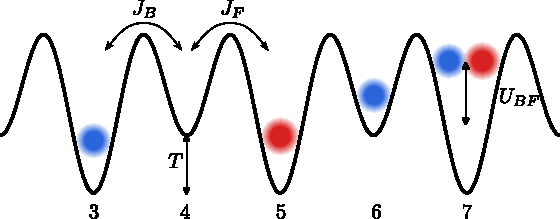
\includegraphics[width=0.5\linewidth]{./images/staggered_lattice_poster.pdf}
			\captionsetup{type=figure}
			\vspace{-10pt}
			\caption{\textbf{Schematic depiction of the system.}\\ Bosons (blue) and fermions (red) in a 1D lattice. The bosonic (fermionic) coherent tunneling at strength $J_B$ ($J_F$) is described by the operator $V$ in \eqref{eq:new_heff}.
			The bosons are subject to a staggered potential of strength $T$ which enhances (lowers) their energy at even (odd) sites and interact with the fermions with strength $U_{BF}$, which is described by $H_0$ in \eqref{eq:new_heff}.} 
			% and depictied in the right half of the sketch.}
		\end{figure}
	\end{figure}

	\addtocounter{figure}{-2}
	\begin{figure}[H]
		\section{Effective Hamiltonian}
		\begin{AutoMultiColEnumerate}
			\item Consider the limit $J_B,J_F\ll U_{BF},T\Rightarrow V$ can be viewed as a perturbation to $H_0$.
			\item Transform $V$ into interaction picture via $U=e^{-iH_0t}$
			\begin{equation*}
			V^I(t)=U^\dagger V U.
			\end{equation*}
			\item Tune onsite potential $T$ on resonance with the boson-fermion interaction $U_{BF}$: $T=U_{BF}$.
			\item Apply a rotating-wave approximation (RWA), i. e. keep only time-independent terms in $V^I(t)$.
		\end{AutoMultiColEnumerate}
		\begin{shaded}
			\textbf{Effective Hamiltonian}
			\begin{equation}
				H_{eff}=-J_B\sum_{j\text{ odd}}(\bdag{j}\bos{j+1}\overline{\Prj_{j+1}^F}+\bdag{j}\bos{j-1}\overline{\Prj_{j-1}^F}+h.c.)\Prj_{j}^F
						-J_F\sum_j (\cdag{j}\fer{j+1}+h.c.)\Prj_{j+1=j}^B
			\label{eq:new_heff}
			\end{equation}

			$\rightarrow\ \Prj_{j}^F=\cdag{j}\fer{j}$ is the projector onto the subspace of Fock states containng a fermion at site $j$ and $\overline{\bullet}$ denotes the projector onto the complement\\
			$\rightarrow\ \Prj_{j+1=j}^B=\sum_{n=0}^\infty\ketbra{n}{n}_j\otimes\ketbra{n}{n}_{j+1}$ is the projector onto the subspace of Fock states of equal boson occupation number at site $j$ and $j+1$
		\end{shaded}

		% \begin{itemize}
		% \item The dynamics described by \eqref{eq:new_heff} can be understood in terms of elementary processes illustrated in \figref{fig:el_proc}
		% \end{itemize}
		\vspace*{+25pt}
		\begin{minipage}{0.48\textwidth}
			\textit{Fermion hopping under kinetic constraint}
			\begin{itemize}
				\item In \figref{fig:el_proc} a (b) fermion hopping between sites $j$ and $j-1$ is allowed as both sites do (not) contain a boson
				\item In general, hopping is allowed if both sites contain the same amount of bosons, see $\Prj_{j+1=j}^B$ in \eqref{eq:new_heff}.
			\end{itemize}
			\textit{Boson hopping under kinetic constraint}
			\begin{itemize}
				\item In the fermion configurations of \figref{fig:el_proc} c (d) boson hopping between an odd site $k$ and its left (right) neighbor is allowed 
				\item Those hopping processes are mathematically described by the terms $~J_B$ in \eqref{eq:new_heff}.
			\end{itemize}
		\end{minipage}
		\hspace*{+50pt}
        \begin{minipage}{0.42\linewidth}
			\begin{figure}
                 \centering
                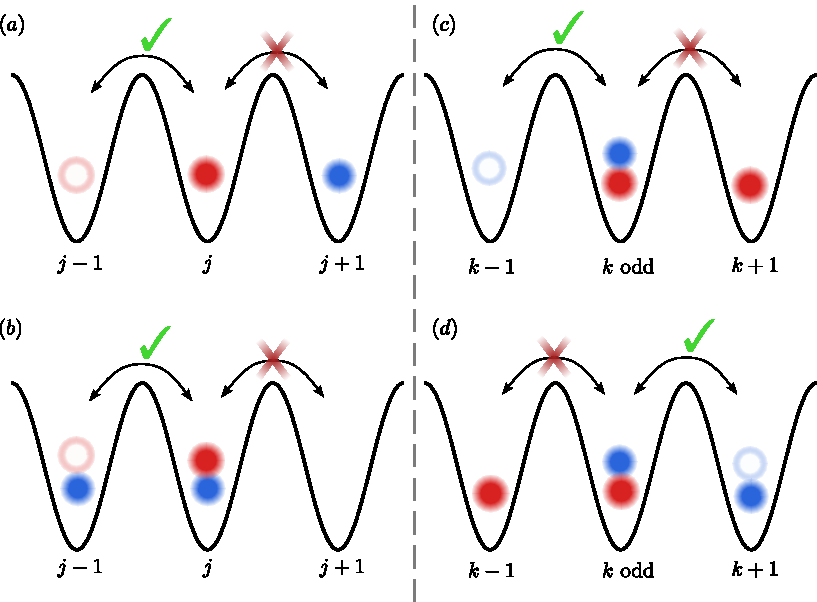
\includegraphics[width=\linewidth]{./images/poster_elproc.pdf}
                \captionsetup{type=figure}
                \vspace{-10pt}
                \caption{\textbf{Elementary processes described by $H_{eff}$.} }
				\label{fig:el_proc}
			\end{figure}
    	\end{minipage}
	
	\end{figure}

	\vspace*{-50pt}
	\addtocounter{figure}{-2}
	\begin{figure}[H]
		\section{One fermion in a bosonic background}
		\begin{itemize}
			\item Consider a light fermion immersed in background of heavy bosons, $J_B\ll J_F$.
				\begin{AutoMultiColEnumerate}
					\item Derive Heisenberg equations of motion (EOM) for the bosonic ladder operators from \eqref{eq:new_heff}.
					\item Apply \textit{Born-Oppenheimer} approximation (BO) using the seperation of time scales $J_B\ll J_F.$
					% hence tracing over 
					% the bosonic degrees of freedom (DOF) in \eqref{eq:new_heff} $\rightarrow$ $L$ dimensional fermionic Hamiltonian ($L=$ system size)
					\item Take expectation values over Heisenberg EOM using BO to decouple fermionic and bosonic DOFs $\langle ...\rangle_{B+F}\approx\langle...\rangle_B\langle...\rangle_F$. 
					\item Apply \textit{Mean-field} approximation (MF) : $\ket{\Psi}_B \approx \ket{\alpha}_1\otimes\ket{\alpha}_2\otimes...\otimes\ket{\alpha}_L \Rightarrow \langle \bdag{j}\bos{j+1}\rangle\approx \langle b_j\rangle^* \langle b_{j+1}\rangle$ with coherent states $\ket{\alpha_j}$ and mean occupation $n_j=|\alpha_j|^2$. 
				\end{AutoMultiColEnumerate}
			% \item[$\Rightarrow$] semiclassical description: fermionic one particle wave function $\ket{\Psi}_F$ evolving under $H_{eff}^F$ coupled to time-dependent bosonic mean field amplitudes.
		\end{itemize}
		\begin{shaded}
			\textbf{System of coupled equations}\\
				MF equations of motion for bosonic amplitudes
				\begin{equation}
				\begin{aligned}
				i \frac{d}{dt}\bos{j}=& -J_B \begin{cases}
								(\bos{j+1} + \bos{j-1})\left|\braket{j}{\Psi}_F\right|^2 & j\text{ odd},\\
								\bos{j+1}\left|\braket{j+1}{\Psi}_F\right|^2 + \bos{j-1}\left|\braket{j-1}{\Psi}_F\right|^2 & j\text{ even}
								\end{cases}\\
								& -J_F\left(\left(\braket{\Psi}{j}\braket{j+1}{\Psi}_F+c.c.\right)\langle B_1\rangle_B + \left(\braket{\Psi}{j-1}\braket{j}{\Psi}_F+c.c.\right)\langle B_2\rangle_B\right).
				\end{aligned}
				\label{eq:mf_bos_eom}
				\end{equation}

				Schrödinger equation for the fermionic one-particle wave function $\ket{\Psi}_F$ evolving under $H_{eff}^F$
					\begin{equation}
						i \frac{d}{dt}\ket{\psi}_F = H_{eff}^F \ket{\psi}_F,\ H_{eff}^F = - J_B \sum_{j \text{ odd}} \left(|b_j^* b_{j+1}|^2+|b_j^*b_{j-1}|^2\right) \ketbra{j}{j}_F
									- J_F \sum_j \langle\Prj_{j+1=j}^B\rangle_B (\ketbra{j}{j+1}_F+h.c.).
						\label{eq:schroedinger_ferm}
					\end{equation}

			\end{shaded}
		% \begin{figure}
		% 	%\vspace*{-75pt} %rand von bild entfernen
		% 	\centering
		% 	\includegraphics[width=0.5\textwidth]{./images/DemoPlot.png}
		% 	%\vspace*{-120pt} %rand von bild entfernen
		% \end{figure}
	\end{figure}

	% \addtocounter{figure}{-2}
	% \begin{figure}
	% 	\section{Collective approach: Master equation}
	% 	Derive the master equation in presence of nearest neighbour interactions \cite{Gonzalez2017}.\\
	% 	We proceed analogously to \cite{Breuer_2007,lidar2020lecture,Schaller2015} and obtain \eqref{eq:masterCollective}.
	% 	\begin{align}
	% 		H & =
	% 		\ot{
	% 		\ut{\omega_a\sum_k{n_k}}{bare atom energy}
	% 		\textcolor{rot}{+\ut{V \sum_k{n_kn_{k+1}}}{Rydberg interaction}}
	% 		+\ut{\sum_q{\omega_q a_{q}^\dagger a_q}}{bath energy}
	% 		}{$H_0$}
	% 		+\ut{\sum_{q,k}{g_{qk}(a_q \e^{\i \vb{q \cdot r}_k}+a_{q}^\dagger\e^{-\i \vb{q \cdot r}_k})\sigma_k^x}}{system-bath interaction}
	% 		\label{eq:HamiltonMitBad}
	% 	\end{align}
	% \end{figure}
	% \addtocounter{figure}{-2}
	% \begin{figure}
	% 	\begin{AutoMultiColEnumerate}
	% 		\item transform into interaction picture via unitary\\ $U=\text{exp}(\i H_0 t)$
	% 		\item apply Born-Markov approximation
	% 		\item apply rotating-wave approximation
	% 		\item assume large Rydberg interaction $V/\gamma\gg 1$
	% 		\item define the configuration dependent decay rate $\Gamma^\xi$ with dipole matrix element $\vb{d_{gs}}=\mel**{g}{e\vb{r}}{s}$
	% 		\begin{equation}
	% 			\Gamma^\xi =
	% 			\frac{\abs{\vb{d_{gs}}}^2}{3 \pi \hbar \epsilon_0 c^3}
	% 			(\omega_a+\xi V)^3
	% 			\label{eq:GammaXi}
	% 		\end{equation}
	% 	\end{AutoMultiColEnumerate}
	% \end{figure}
	% \begin{shaded}
	% 	\textbf{Collective master equation}
	% 	\begin{equation}
	% 		\dot\rho_\text{int}  = \mathlarger{\mathlarger{\sum}}_{\xi=\left\{ 0,1,2 \right\}}
	% 		\Gamma^\xi
	% 		\sum_k \ut{\sigma_k P_k^\xi}{$L_k^\xi$} \rho\ P_k^\xi \sigma_k^\dagger
	% 		+ \acomm{ \sigma_k P_k^\xi \sigma_k^\dagger}{\rho}
	% 		\label{eq:masterCollective}
	% 	\end{equation}
	% 	\begin{AutoMultiColItemize}
	% 		\renewcommand\labelitemi{\textcolor{rot}{$\rightarrow$}}
	% 		\item jump operators change to collective jump operators $L_k^\xi=\sigma_k P_k^\xi$
	% 		$\Rightarrow$ dissipation is configuration dependent
	% 		%\item each configuration $\xi$ decays with specific rate $\Gamma^\xi$
	% 	\end{AutoMultiColItemize}
	% \end{shaded}


	\addtocounter{figure}{-1}
	\begin{figure}
		\begin{minipage}{\textwidth}
			\section{2 particles on a ring lattice - dynamically disconnected subspaces}
			\begin{itemize}
				\item Consider a ring lattice with $L$ sites ($L$ even) and periodic boundary conditions occupied by 1 fermion and 1 boson $\rightarrow$ Hilbertspace $\mathcal{H}=\text{span}\{\ket{i}_B\otimes\ket{j}_F=\ket{ij},\ i,j=1,...L\}$, dim($\mathcal{H})=L^2$.
				\item Hilbert space decomposes into $L+1$ dds due to the kinetic constraint, see blue squares in  \figref{fig:dds_sketch} 
				% i. e. for $L\rightarrow\infty$: nr of dds $=\sqrt{\text{dim}(\mathcal{H})}$:
				\item [$\rightarrow$] $L/2$ frozen states \{$\ket{jj}$\}, $j$ even $\leftrightarrow$ both particles immobile
				\item [$\rightarrow$] $L/2$ subspaces $\text{span}\{\ket{ji}\}$, $j$ even, $i\neq j$ with dim=$L-1$ $\leftrightarrow$ boson immobile, fermion mobile
				\item [$\rightarrow$] 1 subspace $\mathcal{D}$ $\leftrightarrow$ both particles move under kinetic constraint, see the large square in  \figref{fig:dds_sketch}
			\end{itemize}
			\begin{figure}
			\centering
			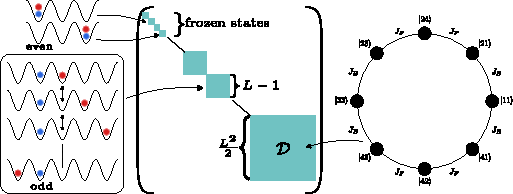
\includegraphics[width=0.5\textwidth]{./images/dds_sketch.pdf}
			\captionsetup{type=figure}
			\vspace{-10pt}
			\caption{\textbf{Structure of the dynamically disconnected subspaces.} The ring structure on the right represents the coupling between Fock states of the projection of $H_{eff}$ onto subspace $\mathcal{D}$, $H_{eff}|_{\mathcal{D}}=\Prj_D H_{eff} \Prj_D$
			for $L=4$.}
			\label{fig:dds_sketch}
			\end{figure}

			% 		\begin{itemize}
			% 			\renewcommand\labelitemi{\textcolor{rot}{$\rightarrow$}}
			% 			\item for the local approach, we assume that the decay rate of an atom is independent of the configuration of its neighbours $\Gamma^\xi=\gamma$
			% 			\item for the collective approach, we assume that the decay rate of an atom depends on the configuration of its neighbours $\Gamma^\xi=\gamma+\xi V$ with $\xi=0,1,2$ being the number of excited neighbours
			% 		\end{itemize}
			% 	\item study the excitation density $\expval{n}$ in the steady stationary state
			% 	%\item use equation of motion formalism \cite{Schaller2015}
			% 	\item apply mean-field approximation $\expval{n \sigma_x}=\expval{n}\expval{\sigma_x}$ and homogenize atoms$\expval{n_k}=\expval{n_{k'}}$ \cite{PhysRevLett.101.250601}
			% \end{itemize}
	% 		\begin{itemize}
	% 			\renewcommand\labelitemi{\textcolor{rot}{$\rightarrow$}}
	% 			\item \textcolor{rot}{for the collective approach we obtain an additional summand $4\expval{n}$ (in red)} in the system of equations \eqref{eq:mean-field}, which comes from the entry of the neighbouring atoms
	% 			\item depending on chosen parameters $\Omega$ and $\Delta$ either 1 or 3 solutions result
	% 			\item either 1 or 2 are stable $\rightarrow$ study only those
	% 		\end{itemize}
	% 		\begin{minipage}[c][][t]{0.54\textwidth}
	% 			\begin{shaded}
	% 				\textbf{System of equations}
	% 				\begin{alignat}{7}%[leftmargin=0pt]
	% 					 & \expval{\dot{n}}        &  & =  & \Omega \expval{\sigma_y} & - \gamma \expval{n}                                                           &  &                                   &  & \nonumber             \\
	% 					 & \expval{\dot{\sigma}_x} &  & =- & \Delta \expval{\sigma_y} & -\frac{\gamma}{2}(\mathbin{\textcolor{rot}{4\expval{n}}}+1) \expval{\sigma_x} &  & -2 V \expval{n} \expval{\sigma_y} &  & \label{eq:mean-field} \\
	% 					 & \expval{\dot{\sigma}_y} &  & =- & \Delta \expval{\sigma_x} & -\frac{\gamma}{2}(\mathbin{\textcolor{rot}{4\expval{n}}}+1)\expval{\sigma_y}  &  & +2 V \expval{n} \expval{\sigma_x} &  & \nonumber             \\ %[-1.5em]
	% 					 &                         &  &    &                          & -2\Omega (2\expval{n} -1)                                                     &  &                                   &  & \nonumber
	% 				\end{alignat}
	% 			\end{shaded}
	% 		\end{minipage}
	% 		\hfill
	% 		\begin{minipage}[c][][t]{0.44\textwidth}
	% 			\captionsetup{type=figure}
	% 			\centering
	% 			\vspace*{-10pt} % Remove white border on top of plot
	% 			\includegraphics[width=\textwidth]{./images/DemoPlot.png}
	% 			\vspace*{-60pt} % Remove white border under plot
	% 			\caption{
	% 				\textbf{Number of solutions with the collective approach $(c)$, the local approach $(l)$.}
	% 				We set $V=10\gamma$. We observe a shift in phase boundaries and critical points.}
	% 			\label{fig:NofSols}
	% 		\end{minipage}
	  	\end{minipage}
	  \end{figure}

	% \addtocounter{figure}{-2}
	% \begin{figure}
	% 	\begin{minipage}[t]{0.5\textwidth}
	% 		\begin{figure}
	% 			\captionsetup{type=figure}
	% 			\centering
	% 			\vspace*{-60pt}
	% 			\includegraphics[width=\textwidth]{./images/DemoPlot.png}
	% 			%\vspace*{-60pt} % weißen Rand vom Plot entfernen
	% 			\caption{\textbf{Excitation density phase diagrams for collective and local approach.} $V=10\gamma$.
	% 				The low density solution corresponds to the smallest of the 3 solutions, the high density to the largest. We observe a shift in the phase boundaries for both solutions.
	% 			}
	% 			\label{fig:AbsSols}
	% 		\end{figure}
	% 	\end{minipage}
	% 	\hfill
	% 	\begin{minipage}[t]{0.47\textwidth}
	% 		\captionsetup{type=figure}
	% 		\centering
	% 		\vspace*{-16pt}
	% 		\includegraphics[width=\textwidth]{./images/DemoPlot.png}
	% 		\vspace*{-40pt} % weißen Rand vom Plot entfernen
	% 		\caption{\textbf{Relative deviation of the phase diagrams} with collective vs. the local approach. We set $V=10\gamma$.	The low density solution corresponds to the smallest of the 3 solutions, the high density to the largest. In the area of the transitions from \figref{fig:NofSols} we find a high relative deviation here.}
	% 		\label{fig:DiffofSols}
	% 	\end{minipage}
	% \end{figure}

	% \addtocounter{figure}{-2}
	% \begin{figure}[h]
	% 	\begin{minipage}{0.55\textwidth}
	% 		\section*{Relative deviation for finite number of particles}
	% 		\begin{itemize}
	% 			\item for particle numbers $N<6$, we use the method of exact diagonalization
	% 			      % by means of the Choi-Jamilkowski formalism
	% 			      \cite{Schaller2015}. For $N\geq6$, we use the \glqq continuous-time Monte Carlo\grqq\ algorithm from \cite{Plenio1998}.
	% 			\item simulations are done with Python framework QuTiP \cite{qutip1,qutip2}.
	% 			\item[\textcolor{rot}{$\rightarrow$}] in \figref{fig:numericResults} similar parameter regimes for differences compared to the mean-field calculations can be identified
	% 			\item[\textcolor{rot}{$\rightarrow$}] clear differences for $\Delta/ \gamma<-5$: Excitation density is higher for the collective approach
	% 			\item periodic effects in Monte Carlo calculations are most likely due to residual oscillations of the equilibrium state after finite simulation time
	% 		\end{itemize}
	% 	\end{minipage}
	% 	\hfill
	% 	\begin{minipage}{0.4\textwidth}
	% 		\begin{figure}
	% 			\captionsetup{type=figure}
	% 			\vspace*{-50pt} % remove whitespace on top of plot
	% 			\includegraphics[width=\linewidth]{./images/DemoPlot.png}
	% 			\vspace*{-60pt}
	% 			\caption{\textbf{Relative deviation of phase diagrams with finite number of particles $N$} at $V=10\gamma$. Normalized by the number of particles.}
	% 			\label{fig:numericResults}
	% 		\end{figure}
	% 	\end{minipage}
	% \end{figure}

	\section{Conclusion and outlook}
	\begin{AutoMultiColItemize}
		\renewcommand\labelitemi{\textcolor{rot}{$\rightarrow$}}
		\item in the limit of a light fermion immersed in a background of non-interacting heavy bosons, we derived a MF description using BO approximation
		\item [$\rightarrow$] dynamics dependent on initial state (ballistic $\leftrightarrow$ immobile), effective background potential caused by bosons leads to fermion distribution over sublattice
		\item [$\rightarrow$] fermion movement suppressed for high boson densities 
		\item extend MF analysis to a 2D lattice
		\item perform systematic analysis of the spectrum of $H_{eff}$ based on the observation of the dds for 2 particles $\rightarrow$ candidate for HSF?
		\item consider hardcore boson limit $U_{BB}\rightarrow \infty$
	\end{AutoMultiColItemize}
\end{multicols}

\vspace*{+100pt}
\textcolor{rot}{\rule{\textwidth}{4pt}}
\setlength{\columnseprule}{0pt}
\begin{multicols}{2}
	\vspace*{-70pt}
	\printbibliography[heading=customBibTitle]
	\vspace*{-10pt}

	\section*{Contacts}
	{\small
		Felix Stephan\\
		felix.stephan@student.uni-tuebingen.de\\
		Auf der Morgenstelle~14\\
		72076~Tübingen, Germany
	}
\end{multicols}
\end{document}
